
\begin{figure}
    \centering
    \begin{subfigure}[c]{0.45\textwidth}
        \centering    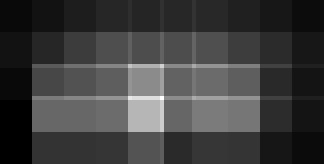
\includegraphics[scale=2.0]{resources/MNIST_soft_att/1177_att.jpg}
        \caption{Soft attention in white on the image to the right. It correctly focuses more to the bottom and left.}
        % \label{fig:mnist_early_models}
    \end{subfigure} \quad %
    \begin{subfigure}[c]{0.45\textwidth}
        \centering
        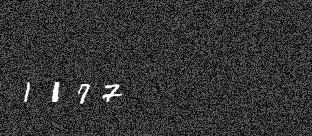
\includegraphics[scale=2.0]{resources/MNIST_soft_att/1177_correct.jpg}
        \caption{The image is correctly classified as 1177.}
        % \label{fig:mnist_models}
    \end{subfigure}
    
    \begin{subfigure}[c]{0.45\textwidth}
        \centering    
\includegraphics[scale=2.0]{resources/MNIST_hard_att/1281_att.jpg}
        \caption{Hard attention in white of the image to the right. The attention only captures part of the number.}
        % \label{fig:mnist_early_models}
    \end{subfigure} \quad %
    \begin{subfigure}[c]{0.45\textwidth}
        \centering
        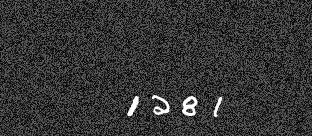
\includegraphics[scale=2.0]{resources/MNIST_hard_att/1281_fail_1031.jpg}
        \caption{Input image with label 1281, it was incorrectly classified as 1031.}
        % \label{fig:mnist_models}
    \end{subfigure}
    \caption{Examples of soft and hard attention applied to noisy MNIST images with sizes $312 \times 136$.}
\end{figure}